\newpage % Rozdziały zaczynamy od nowej strony.
\section{Przeglad }
W rozdziale tym dokonuje przeglądu istotnych zagadnień związanych z zarządzaniem łańcuchem dostaw oraz uczeniem maszynowym. Przedstawimy definicje, teorie, rodzaje  zarządzania łańcuchem dostaw  i maszynowego uczenia . Następnie omówiam definicje i zastosowania maszynowego uczenia w zarządzaniu łańcuchem dostaw.


\subsection{Zarządzania łańcuchem dostaw}
W niniejszym podrozdziale dokładnie omówiam najważniejsze zagadnienia związane z zarządzaniem łańcuchem dostaw( definicje, cele oraz znaczenie) . Ponadto wyjaśniam z jakich elementów składa się zarządzanie łańcuchem dostaw.

\vspace{\baselineskip}
\subsubsection{Definicje Zarządzania Łańcuchem Dostaw} 
\vspace{\baselineskip}
\textbf{Definicje z różnych źródeł:}

Zarządzanie łańcuchem dostaw (ang. Supply Chain Management, SCM) jest kompleksowym podejściem do planowania, kontrolowania i monitorowania wszystkich procesów związanych z dostarczaniem produktów lub usług od dostawców do klientów końcowych. Jest to obszar, który obejmuje wiele etapów, począwszy od zaopatrzenia, produkcji, dystrybucji, aż po dostarczenie produktu lub usługi do ostatecznego użytkownika.

Zarządzanie łańcuchem dostaw (ang. Supply Chain Management – SCM) – zarządzanie przepływami między ogniwami łańcuchem dostaw. Umożliwia projektowanie, planowanie, realizację, kontrolę oraz monitoring łańcucha dostaw. \cite{wik2023}



Wg. Encyklopedii zarzadzania Łańcuch dostaw - obejmuje wszelkie czynności związane z transportem oraz przeróbką towarów, wspominając tutaj również o początkowym etapie, czyli pozyskiwaniu wszelkiego rodzaju surowców oraz etapie końcowym tj. dostarczeniu produktu konsumentom. Pojęcie to zawiera również przepływ informacji, które są istotne podczas całego procesu. \cite{zarz2023}

Zarządzanie łańcuchem dostaw obejmuje wszystkie działania, które przekształcają surowce w gotowe produkty i oddają je w ręce klientów. Może to obejmować określanie źródła dostaw, projektowanie, produkcję, magazynowanie, wysyłkę i dystrybucję. Celem SCM jest poprawa wydajności, jakości, produktywności i zadowolenia klientów. \cite{scm2023}

Łańcuch dostaw jest to skoordynowana sieć wzajemnych powiązań logistyczno - operacyjnych, która obejmuje wszelkie firmy, obiekty i działania biznesowe zaangażowane w pozyskiwanie, opracowywanie, wytwarzanie i dostarczanie produktów.
Każda firma tworzy swój własny łańcuch dostaw, aby móc wytwarzać produkty i wprowadzać je na rynek. Może również sama być ogniwem w łańcuchach dostaw innych firm. Działania łańcucha dostaw przekształcają zasoby naturalne, surowce i komponenty w gotowy produkt, który jest dostarczany do użytkownika końcowego. \cite{wdx2023}

 (SCM) zajmuje się systemem zakupów (zakup surowców/komponentów), zarządzaniem operacyjnym (zapewnienie produkcji wysokiej jakości produktów z dużą szybkością, dobrą elastycznością i niskimi kosztami produkcji), logistyką i kanałami marketingowymi , dzięki któremu surowce można przekształcić w gotowe produkty i dostarczyć klientom końcowym.Węższa definicja zarządzania łańcuchem dostaw to „projektowanie, planowanie, realizacja, kontrola i monitorowanie działań w łańcuchu dostaw w celu tworzenia wartości netto, budowania konkurencyjnej infrastruktury, wykorzystania światowej logistyki, synchronizacji podaży z popytem i pomiaru wydajności globalnie”. Może to obejmować przemieszczanie i przechowywanie surowców, zapasów w toku, wyrobów gotowych i kompleksową realizację zamówień od punktu pochodzenia do punktu konsumpcji. \cite{wiken2023}

\vspace{\baselineskip}
\textbf{Historia}
Łańcuchy dostaw istnieją od czasów starożytnych, poczynając od pierwszego wytworzonego i sprzedanego produktu. Wraz z nadejściem industrializacji zarządzanie łańcuchem dostaw stało się bardziej złożone i pozwoliło przedsiębiorstwom na efektywniejsze wytwarzanie i dostarczanie towarów i usług. Na przykład wprowadzona przez Henry'ego Forda standaryzacja części samochodowych okazała się przełomem, który pozwolił na masową produkcję towarów, aby sprostać wymaganiom rosnącej liczby klientów. Z biegiem czasu kolejne zmiany (takie jak wprowadzenie na rynek komputerów) systematycznie zwiększały poziom zaawansowania systemów SCM. Systemy te pozostawały jednak przez wiele lat zasadniczo liniową, autonomiczną funkcją zarządzaną przez specjalistów ds. łańcucha dostaw. 
Sytuacja zmieniła się diametralnie wraz z pojawieniem się Internetu, innowacji technologicznych i gospodarki globalnej opartej na popycie. Obecnie zarządzanie łańcuchem dostaw nie jest już funkcją liniową, ale raczej złożonym zbiorem niejednorodnych sieci dostępnych całodobowo. W centrum tych sieci znajdują się konsumenci oczekujący realizacji swoich zamówień w wybrany przez nich sposób.\cite{oracle2023}

\vspace{\baselineskip}
\textbf{Pochodzenie terminu}.W 1982 roku Keith Oliver, konsultant w firmie Booz Allen Hamilton, w wywiadzie dla Financial Times wprowadził do domeny publicznej termin „zarządzanie łańcuchem dostaw”. W 1983 roku WirtschaftsWoche w Niemczech opublikowało po raz pierwszy wyniki wdrożonego tzw. „projektu zarządzania łańcuchem dostaw”, kierowanego przez Wolfganga Partscha.
W połowie lat 90. termin „zarządzanie łańcuchem dostaw” zyskał na popularności, gdy ukazała się lawina artykułów i książek na ten temat. Pierwotnie łańcuchy dostaw zdefiniowano jako obejmujące wszystkie działania związane z przepływem i przetwarzaniem towarów od surowców do użytkownika końcowego lub konsumenta końcowego, a także powiązane przepływy informacji. Mentzer i in. uważają za godne odnotowania, że te wcześniejsze definicje obejmowały konsumenta końcowego. Zarządzanie łańcuchem dostaw zostało następnie zdefiniowane jako integracja działań w łańcuchu dostaw poprzez ulepszone relacje w łańcuchu dostaw w celu osiągnięcia przewagi konkurencyjnej. \cite{wiken2023}


\vspace{\baselineskip}
\subsubsection{Cele Zarządzania Łańcuchem Dostaw}



Najczęściej opisywanymi celami łańcucha dostaw w ujęciu logistycznym jest:

  \par - Minimalizacja kosztów wynikających z przepływu towarów i informacji przy zachowaniu dobrego poziomu obsługi klienta
  \par - Krótki czas realizacji zamówień oraz bezproblemowość i elastyczność dostaw
   \par- Optymalizacja poziomu zapasów wraz z dostosowaniem się do potrzeb rynku \cite{zarz2023}


Podsumowujac: Głównym celem zarządzania łańcuchem dostaw jest zapewnienie, że produkty lub usługi są dostarczane w odpowiednim czasie, w optymalnych ilościach, przy minimalnych kosztach oraz z zachowaniem wysokiej jakości. SCM dąży do zintegrowania wszystkich elementów łańcucha dostaw, tak aby procesy były bardziej efektywne i konkurencyjne.

Ale wazne aby odnotować zmiane w celach ..raczej ktore cele sa obecnie najwazniejsze:
Dzisiejsze systemy SCM są całkowicie ukierunkowane na klienta
Celem zarządzania łańcuchem dostaw zawsze było zwiększanie efektywności i obniżanie kosztów. Cele te nie uległy zmianie, ale obecnie główną rolę w ustalaniu priorytetów takiego zarządzania odgrywa klient. Mówi się, że „doświadczenia klientów żyją i umierają w łańcuchu dostaw”.
Lojalność klientów zależy od tego, czy przedsiębiorstwo jest w stanie szybko i dokładnie spełnić ich oczekiwania. Dostawy surowców, produkcja, logistyka, sprzedaż i zarządzanie zamówieniami muszą być ze sobą skoordynowane, aby klient otrzymał to, co chce, w rozsądnym terminie. W tym celu przedsiębiorstwo musi analizować swoje łańcuchy dostaw z perspektywy klientów. Nie chodzi tu bowiem tylko o terminową dostawę, ale również o wykonanie we właściwym czasie wszystkich niezbędnych czynności, zarówno przed taką dostawą, jak i w jej trakcie oraz po jej zrealizowaniu.\cite{oracle2023}


\vspace{\baselineskip}
\subsubsection{Znaczenie zarządzania Łańcuchem Dostaw}

Łańcuchy dostaw zawsze były napędzane przez wiele sił globalnych i politycznych, a nawet przez warunki pogodowe i wydarzenia naturalne. Jest jednak jedna rzecz, która jest pewna w zarządzaniu łańcuchem dostaw i to jest zmiana. 
Nowoczesna logistyka stawia menedżerów przed wieloma wyzwaniami skutecznej organizacji łańcuchów dostaw, optymalizacji kosztów i zarządzania stanami magazynowymi. Wszystko to ułatwią rozwijające się technologie Łańcuchów Dostaw 4.0. To szerokie pojęcie obejmuje między innymi zastosowanie IoT w logistyce, użycie zaawansowanej robotyki w magazynach oraz zaawansowaną analizę Big Data, a nawet sztuczną inteligencję. Dzięki czujnikom, sieciom, nowoczesnemu oprogramowaniu i automatyzacji możliwe jest nie tylko zwiększenie skuteczności procesów logistycznych, ale także ograniczenie kosztów oraz wyższy poziom zadowolenia klienta z dostaw.
Znaczenie systemów SCM: Istota zarządzania łańcuchem dostaw
Wystarczy się rozejrzeć. Wszystko, co znajduje się w Twoim domu lub zakładzie pracy, trafiło tu dzięki łańcuchom dostaw. Działania te wymagają zaangażowania pracowników z milionów miejsc pracy na całym świecie. Przez łańcuch dostaw przewija się wszystko — od tanich dóbr konsumpcyjnych aż po przyrządy chirurgiczne i kluczowe zasoby. Wciąż jednak, mimo iż zarządzanie łańcuchami dostaw leży u podstaw gospodarki światowej, wiele organizacji korzysta w tym celu z procesów i maszyn stosowanych od 50 lat.\cite{scm2023}

  Wiele firm po prostu przestałoby działać bez zarządzania łańcuchem dostaw, więc to dość duże korzyści SCM.  Niektóre z zalet zoptymalizowanego zarządzania łańcuchem dostaw obejmują: 

   - Większa produktywność: systemy do zarządzania zasobami przedsiębiorstwa i przeglądy zapobiegawcze zwiększają wydajność maszyn i systemów. Może to pomóc w wyeliminowaniu wąskich gardeł, usprawnieniu procesów i zwiększeniu produktywności. Zautomatyzowane procesy i responsywne analizy danych przekładają się na szybszy transport i krótszy czas dostawy.
   
   -Niższe koszty łańcucha dostaw: przy użyciu analiz predykcyjnych można wyeliminować konieczność szacowania w oparciu o przypuszczenia. Pozwoli to ograniczyć zarówno marnotrawienie zapasów, jak i ryzyko ich deficytu. Internet rzeczy zapewnia większą responsywność istniejących zasobów oraz maksymalnie wydajny i praktyczny przepływ pracy w każdej sytuacji. Bardziej precyzyjne prognozy umożliwiają ponadto redukcję liczby niezaładowanych w pełni samochodów dostawczych i nieskoordynowanych tras dostaw, a także bardziej efektywne zarządzanie flotą.
   
   - Większa elastyczność i odporność łańcucha dostaw: Trendy i zmiany na rynku mogą nastąpić nagle. Odporne systemy SCM są elastyczne, aby dostosować się do każdej sytuacji. Dane w czasie rzeczywistym i inteligentne analizy mogą pomóc menedżerom łańcucha dostaw przenieść maszyny i personel do lepszych przepływów pracy. Opinie klientów można od razu usłyszeć i podjąć odpowiednie działania. Wirtualne zapasy i inteligentne procesy magazynowe zapewniają dostosowanie podaży i popytu.
   
   -Wyższa jakość produktów: zapewnienie zespołom ds. badań i rozwoju dostępu do informacji zwrotnych od klientów sprawia, że podczas projektowania i opracowywania produktów brane są pod uwagę ich potrzeby. Zarówno zespół ds. badań i rozwoju, jak i zespół ds. produkcji mogą wykorzystać informacje dostępne dzięki uczeniu maszynowemu i analizom, aby reagować na trendy i oczekiwania klientów oraz doskonalić projekty produktów.
    
    -Lepsza obsługa klienta: najlepsze praktyki SCM są zorientowane na klienta i zaprojektowane tak, aby były responsywne i adaptacyjne. Dzięki konkurencji tylko jednym kliknięciem, nowoczesny SCM pozwala firmom wdrażać opinie klientów i trendy, umożliwiając zarówno mikrorealizację, jak i personalizację na dużą skalę.
    
    -Większa przejrzystość i zrównoważony rozwój: SCM umożliwia pełną przejrzystość, od etapu projektowania i produkcji po logistykę, dostawę i zwroty. Dzięki możliwości wglądu we wszystkie dane wejściowe i wyjściowe w całym łańcuchu organizacje mogą znacznie poprawić swój wpływ na środowisko, często współpracując w tym celu bezpośrednio z dostawcami i innymi dostawcami. \cite{scm2023}

 

\vspace{\baselineskip}
\subsubsection{Składniki Efektywnego Zarządzania Łańcuchem Dostaw}



Elementy łańcucha dostaw

Istnieje pięć elementów tradycyjnych systemów zarządzania łańcuchem dostaw:

    -Planowanie. Planowanie i zarządzanie wszystkimi zasobami wymaganymi do zaspokojenia zapotrzebowania klientów na produkt lub usługę firmy. Po ustanowieniu łańcucha dostaw należy określić mierniki, które pozwolą zmierzyć czy łańcuch dostaw jest wydajny, efektywny, zapewnia wartość klientom i spełnia cele firmy.
    
   - Zaopatrzenie. Wybór dostawców kwalifikowanych, którzy zapewnią towary i usługi potrzebne do stworzenia produktu. Należy również ustalić procesy monitorowania i zarządzania relacjami z dostawcami. Kluczowe działania w tych procesach obejmują zamawianie, przyjmowanie, zarządzanie stanami magazynowymi oraz realizację płatności dla dostawców.
    
   - Produkcja. Czynności wymagane do przyjęcia surowców, wytworzenia produktu, badania jakości, opakowania do wysyłki i przygotowania harmonogramu dostaw.
    
   - Dostawa i logistyka. Koordynacja zamówień klientów, magazynowanie, planowanie dostaw, wysyłka towarów, wystawianie faktur i odbieranie płatności.
    
   - Zwroty. Stworzenie procesu odbioru wadliwych, nadmiarowych lub niechcianych produktów\cite{wdx2023}



Aleksander Wielki powiedział kiedyś słynnie: „Moi logistycy nie mają poczucia humoru… ponieważ wiedzą, że jeśli moja kampania się nie powiedzie, są pierwszymi, których zabiję”. I choć ten przykład jest trochę skrajny, niemniej jednak ilustruje on, jak ważne dla cywilizacji ludzkiej były zawsze łańcuchy dostaw. Efektywne i odporne narzędzia i praktyki w zakresie zarządzania łańcuchem dostaw są niezbędnym elementem przetrwania i sukcesu firmy. Niektóre z podstawowych procesów SCM obejmują:   

    -Planowanie łańcucha dostaw to proces przewidywania popytu na produkty i koordynowania powiązań w łańcuchu dostaw w celu jego realizacji. Oprócz prognozowania popytu i planowania obejmuje on planowanie dostaw, planowanie potrzeb materiałowych (MRP), planowanie produkcji, planowanie sprzedaży i produkcji (SOP)i inne. 

   - Zarządzanie cyklem życia produktu (PLM) to proces zarządzania produktem przez cały jego cykl życia – od ideacji, inżynierii i projektowania po produkcję, serwis i utylizację (lub recykling).

    -Nabycie to proces nabywania materiałów, towarów i usług w celu zaspokojenia potrzeb biznesowych i zapewnienia jakości, uczciwej ceny i wartości tych towarów. Głównym wyzwaniem dla zespołów s. zaopatrzenia i określania źródła dostaw jest przewidywanie dokładnych wolumenów zamówień, ponieważ zarówno niedobory, jak i nadwyżki mogą być szkodliwe dla firmy. 

   - Zarządzanie logistyką to transport i składowanie towarów od początku łańcucha dostaw, z surowcami i produkcją, po dostawę gotowych produktów do sklepów lub klientów – a nawet do obsługi produktów, zwrotów i recyklingu. Funkcje biznesowe obejmują zarządzanie transportemprzychodzącym i wychodzącym, zarządzanie flotą, gospodarkę magazynową, kontrolę zapasów i obsługę klienta. 

   - Zarządzanie realizacją produkcji (MES) monitoruje, śledzi, dokumentuje i kontroluje proces wytwarzania towarów. Utrzymuje produkcję i procesy tak szczupłe, jak to tylko możliwe – zachowując (i poprawiając) jakość, zrównoważony rozwój i zadowolenie klientów. 

   - Zarządzanie aktywami przedsiębiorstwa to proces zarządzania aktywami fizycznymi i ich utrzymania w całym łańcuchu dostaw, od robotyki fabrycznej po floty dostaw. Czujniki IoT, łączność maszyna-maszyna (M2M)– poprawiają wydajność, czas pracy, bezpieczeństwo oraz prewencyjną i predykcyjną konserwację. Niektóre połączone zasoby mogą nawet przewidywać naprawy lub awarie i samodzielnie przeprowadzać konserwację — bezpośrednio do określania źródła dostaw i zamawiania części potrzebnych do wydłużenia cyklu życia.\cite{scm2023}






\subsection{Maszynowe Uczenie}

W tym rozdziale omawiamy podstawowe koncepcje i techniki związane z maszynowym uczeniem. Rozpoczynamy od wprowadzenia do sztucznej inteligencji, definiując, czym jest i jakie są jej główne komponenty. Następnie skupiamy się na maszynowym uczeniu, jego znaczeniu i zastosowaniach.


\vspace{\baselineskip}
\subsubsection{Sztuczna Inteligencja (SI)}
\textbf
Sztuczna inteligencja to dziedzina informatyki, która zajmuje się tworzeniem systemów komputerowych zdolnych do wykonywania zadań, które normalnie wymagają ludzkiego myślenia. SI składa się z kilku głównych komponentów, obejmujących:

\textbf {Definicje sztucznej inteligencji}
Sztuczna inteligencja jest tematem obszernym i szeroko omawianym zarówno w sferze naukowej, publicystycznej, jak i politycznej. Są to działania oparte o modelowanie wiedzy, danych i rozwijanie systemów algorytmów oraz mocy obliczeniowych, co w obecnym stanie techniki pozwala na uzyskanie względnie zautomatyzowanego systemu pozyskiwania, przetwarzania i analizy danych, który daje możliwość samoistnego (autonomicznego) ulepszania systemu lub przewidywania zachowań i działań na podstawie analizy zebranych danych i korelacji między nimi, z możliwością wpływu na środowisko zewnętrzne oraz pozostające z nim w interakcji za pomocą sensorów i siłowników. Interakcje te mogą zachodzić mechanicznie lub z udziałem człowieka w cyklu życia sztucznej inteligencji począwszy od etapu kreacji, rozwoju, wdrożenia, stosowania, aż po etap decyzji o wyłączeniu z pracy i utylizacji.\cite{gov2023}


Ponizej podział i schemat zastosowan sztucznej inteligencji wg. raportu "Game-changing technologies: Transforming production and employment in Europe"
\begin{figure}[!h]
    \label{fig:ai}
    \centering 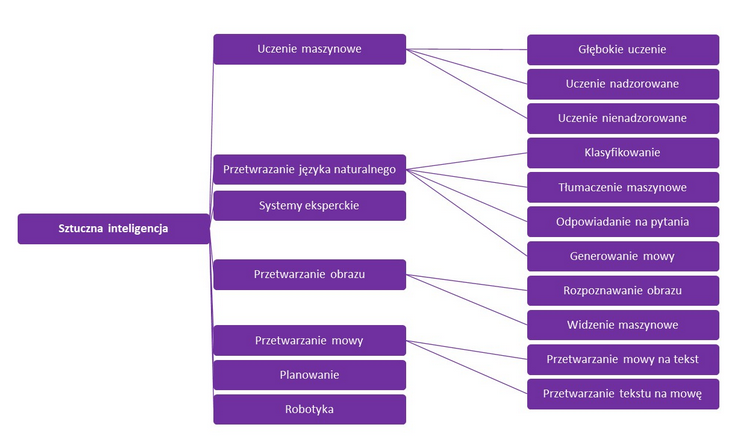
\includegraphics[width=1\linewidth]{AI.png}
    \caption{Obszary zastosowań  sztucznej inteligencji\cite{gov2023}}
\end{figure}

Definicja wg.raportu: "A DEFINITION OF AI:MAIN CAPABILITIES AND DISCIPLINES"  
Sztuczna inteligencja (AI) odnosi się do systemów, które wykazują inteligentne zachowanie poprzez analizę swojego otoczenia i
podejmowanie działań – z pewną dozą autonomii – dla osiągnięcia określonych celów.
Systemy oparte na AI mogą mieć charakter wyłącznie programowy, działać w świecie wirtualnym (np. asystenci głosowi, analiza obrazu
oprogramowanie, wyszukiwarki, systemy rozpoznawania mowy i twarzy) lub sztuczna inteligencja mogą być wbudowane w urządzenia sprzętowe (np.
zaawansowane roboty, samochody autonomiczne, drony czy aplikacje Internetu Rzeczy\cite{ec2029}



\begin{itemize}
    \item \textbf{Uczenie maszynowe (Machine Learning):} Jest to jedna z najważniejszych gałęzi sztucznej inteligencji, która pozwala komputerom na naukę z danych i podejmowanie decyzji na podstawie tych informacji. W ramach uczenia maszynowego wykorzystuje się różne techniki, w tym algorytmy uczenia nadzorowanego i nienadzorowanego.
    
    \item \textbf{Przetwarzanie języka naturalnego (Natural Language Processing - NLP):} Ta dziedzina zajmuje się rozumieniem, przetwarzaniem i generowaniem języka naturalnego przez komputery. NLP jest używane do analizy tekstu, tłumaczenia maszynowego i wielu innych zastosowań.
    
    \item \textbf{Wizja komputerowa:} Obejmuje technologie pozwalające komputerom analizować, rozumieć i interpretować obrazy i wideo. Jest używana w rozpoznawaniu obiektów, rozpoznawaniu twarzy, samochodach autonomicznych i innych dziedzinach.
    
    \item \textbf{Robotyka:} SI jest również istotna w dziedzinie robotyki, gdzie komputery sterują działaniami fizycznymi robotów.
\end{itemize}

\subsubsection{Maszynowe Uczenie}

Maszynowe uczenie (ML) to podzbiór sztucznej inteligencji, który koncentruje się na rozwijaniu algorytmów i technik pozwalających komputerom na naukę z danych i podejmowanie decyzji na podstawie tych informacji. Głównym celem maszynowego uczenia jest rozwijanie modeli, które mogą generalizować zbiory danych i wykonywać zadania bez konieczności programowania ich wprost.

\subsubsection{Zastosowania Maszynowego Uczenia}

Maszynowe uczenie ma szerokie spektrum zastosowań w różnych dziedzinach. W kontekście zarządzania łańcuchem dostaw (SCM), ma to szczególne znaczenie. Poniżej przedstawiamy niektóre z głównych zastosowań ML w SCM:

\begin{itemize}
    \item \textbf{Prognozowanie popytu:} Uczenie maszynowe może być wykorzystywane do prognozowania przyszłego popytu na produkty lub usługi, co pomaga w planowaniu produkcji i zarządzaniu zapasami.
    
    \item \textbf{Optymalizacja zapasów:} Algorytmy ML mogą pomóc w zoptymalizowaniu poziomu zapasów, minimalizując koszty i zapewniając, że dostępność produktów jest na odpowiednim poziomie.
    
    \item \textbf{Wybór dostawcy:} ML może pomóc w analizie dostawców pod kątem efektywności, jakości i kosztów, co ułatwia wybór najlepszego dostawcy.
    
    \item \textbf{Planowanie tras i logistyka:} Algorytmy ML mogą pomóc w optymalizacji tras dostaw, minimalizując czas i koszty transportu.
\end{itemize}

\subsubsection{Rodzaje Maszynowego Uczenia}

Maszynowe uczenie może być podzielone na kilka głównych rodzajów, zależnie od sposobu przetwarzania danych i celu uczenia. Oto niektóre z najważniejszych rodzajów maszynowego uczenia:

\begin{itemize}
    \item \textbf{Uczenie nadzorowane (Supervised Learning):} W tym rodzaju uczenia algorytm jest trenowany na podstawie zestawu danych, który zawiera zarówno wejścia, jak i odpowiadające im oczekiwane wyjścia. Celem jest zbudowanie modelu, który może dokładnie przewidywać wyjście na podstawie nowych danych wejściowych. Przykłady obejmują algorytmy regresji liniowej i klasyfikacji.

    \item \textbf{Uczenie nienadzorowane (Unsupervised Learning):} W przypadku uczenia nienadzorowanego algorytm jest trenowany na danych wejściowych bez oczekiwanych wyjść. Celem jest odkrywanie ukrytych wzorców, grupowanie danych lub redukcja wymiarowości. Przykładem jest klastrowanie danych.

    \item \textbf{Uczenie ze wzmocnieniem (Reinforcement Learning):} Ten rodzaj uczenia polega na trenowaniu agenta, który podejmuje decyzje w środowisku w celu maksymalizacji nagrody. Agent eksploruje różne działania i dostaje informacje zwrotną w postaci nagród lub kar za swoje decyzje. Jest używany w dziedzinach takich jak gry komputerowe i robotyka.

    \item \textbf{Uczenie pół-nadzorowane (Semi-supervised Learning):} Uczenie pół-nadzorowane łączy elementy uczenia nadzorowanego i nienadzorowanego. Model jest trenowany na części danych z etykietami i części danych bez etykiet. Jest stosowane, gdy dostępne są tylko częściowo oznaczone dane.

    \item \textbf{Uczenie głębokie (Deep Learning):} To rodzaj maszynowego uczenia opartego na sieciach neuronowych o wielu warstwach. Jest stosowane do złożonych problemów przetwarzania obrazów, dźwięku i tekstu. Deep Learning osiągnął ogromny sukces w dziedzinach takich jak rozpoznawanie obrazów i przetwarzanie języka naturalnego.

\end{itemize}

Wybór odpowiedniego rodzaju maszynowego uczenia zależy od konkretnego problemu i dostępnych danych. W kontekście zarządzania łańcuchem dostaw, różne rodzaje uczenia maszynowego mogą być stosowane w zależności od konkretnych zadań, takich jak prognozowanie popytu czy optymalizacja tras dostaw.



\subsection{Uczenie maszynowe w zarządzaniu łańcuchem dostaw}
W tym rozdziale dokładniej analizujemy, w jaki sposób maszynowe uczenie może być wykorzystane w zarządzaniu łańcuchem dostaw. Przedstawiamy przykłady konkretnych zastosowań uczenia maszynowego w SCM, takie jak prognozowanie popytu, optymalizacja zapasów czy wybór dostawcy. Omawiamy również korzyści wynikające z wykorzystania tych technik oraz wyzwania, jakie mogą się pojawić.
\subsubsection{Prognozowanie popytu}
Jednym z kluczowych elementów zarządzania łańcuchem dostaw jest zdolność do dokładnego prognozowania popytu na produkty. Maszynowe uczenie oferuje zaawansowane metody analizy danych historycznych oraz czynników wpływających na popyt, co umożliwia dokładniejsze prognozowanie przyszłego zapotrzebowania. Metody te obejmują:

    • Modele szeregów czasowych: Wykorzystują dane historyczne do identyfikowania wzorców w sezonowości i trendach, co pozwala na prognozowanie przyszłego popytu na podstawie danych z przeszłości.
    
    • Algorytmy uczenia maszynowego, takie jak sieci neuronowe i drzewa decyzyjne: Mogą analizować bardziej skomplikowane wzorce w danych, uwzględniając różnorodne zmienne i interakcje między nimi.
    
    • Analiza sentymentu i danych społecznościowych: Wykorzystuje opinię klientów i informacje pochodzące z mediów społecznościowych do oceny wpływu opinii publicznej na popyt na produkty.
    
Precyzyjne prognozy popytu pozwalają firmom lepiej zarządzać swoimi zapasami, minimalizować ryzyko nadmiernego lub niewystarczającego stanu magazynowego oraz dostosować produkcję do rzeczywistych potrzeb rynku.

\paragraph{Modele szeregów czasowych}


Szereg czasowy to ciąg uporządkowanych obserwacji, których dokonuje się w określonych (zwykle stałych) jednostkach czasu. Szeregiem czasowym będzie na przykład średnia cena energii elektrycznej w poszczególnych miesiącach lub ilość zgłaszanych przypadków przemocy domowej w poszczególnych latach. Szereg czasowy można przedstawić w formie wykresu lub tabeli.
Wyróżniamy dwa podstawowe składniki szeregu czasowego – trend i sezonowość. Pojęcie trendu odnosi się do długotrwałej i systematycznej zmiany wielkości danego zjawiska, natomiast sezonowości do rytmicznych, powtarzających się zmian wielkości danego zjawiska, charakteryzujące się różną długością całego cyklu. 
Celem analizy szeregów czasowych jest identyfikowanie i analiza jego struktury, jak również prognozowanie – przewidywanie wartości w kolejnych odstępach czasu, np. sprzedazy. Istnieje wiele metod analizy szeregów czasowych, z czego wiele z nich jest złożonych i obejmują one m.in. analizę trendu (techniki wygładzania) i sezonowości (badanie struktury autokorelacji), modelowanie i prognozowanie szeregów czasowych (m.in. metody ARIMA, wyrównywanie wykładnicze, analiza harmoniczna, analiza widma).\cite{szereg2023}

Szereg czasowy jest bardzo często wykreślany za pomocą wykresu przebiegu (który jest wykresem liniowym czasowym). Szeregi czasowe są wykorzystywane w statystyce, przetwarzaniu sygnałów, rozpoznawaniu wzorców, ekonometrii, finansach matematycznych, prognozowaniu pogody, przewidywaniu trzęsień ziemi,inżynierii sterowania, astronomii, inżynierii komunikacji i głównie w każdej dziedzinie nauk stosowanych i inżynierii, która obejmuje pomiary czasowe.Analiza szeregów czasowych obejmuje metody analizy danych szeregów czasowych w celu wyodrębnienia znaczących statystyk i innych cech charakterystycznych danych. Prognozowanie szeregów czasowych polega na wykorzystaniu modelu do przewidywania przyszłych wartości na podstawie wcześniej zaobserwowanych wartości. Chociaż analizę regresji często wykorzystuje się w celu sprawdzenia zależności między jednym lub większą liczbą różnych szeregów czasowych.W kontekście statystyki, ekonometrii, finansów ilościowych, sejsmologii, meteorologii i geofizyki głównym celem analizy szeregów czasowych jest prognozowanie. W kontekście przetwarzania sygnałów, inżynierii sterowania i inżynierii komunikacji służy do wykrywania sygnału. Inne zastosowania obejmują eksplorację danych, rozpoznawanie wzorców i uczenie maszynowe, gdzie analizę szeregów czasowych można wykorzystać do grupowania, (uwaga od artykulu zrodla!!)[2] [3] klasyfikacji, [4] zapytań według treści, [5] wykrywania anomalii i prognozowania.[6]\cite{series2023}

Poniżej znajdują się elementy szeregu czasowego:
- Sezonowość: Ten element jest powiązany z kalendarzem,  stałe lub okresowe wachania szeregu czasowego zmiennego w czasie,  istnieje a powtarzający się wzór.

- Trend: Ten komponent odnosi się do długoterminowego trendu wartości obserwacji które z czasem mogą się zwiększać lub zmniejszać.

- Cykliczny: Ten składnik odnosi się również do okresowych wcahań czasu serii, ale w odróżnieniu od składnika sezonowości nie jest on stały 

- Losowy: Po wyodrębnieniu wszystkich trzech pozostałych składników z czasu w serii pozostaje element losowy, zwykle ma on strukturę, którą należy zidentyfikować za pomocą modelu w celu dokładnego prognozowania przyszłej wartośi szeregu czasowego.
\cite{Shekh2018}


Mozna wyróżnic wiele modeli szeregów czasowych stosowane do prognozowania :

\begin{figure}[h!]
    \label{fig:S1}
    \centering 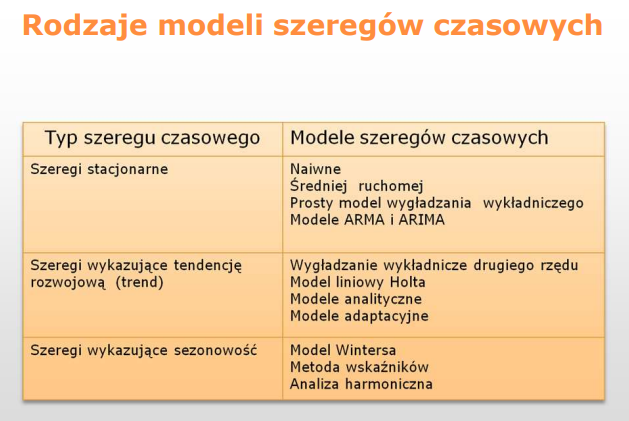
\includegraphics[width=0.5\linewidth]{S1.png}
    \caption{S1 Modele szeregów czasowych\cite{szer2009}}
\end{figure}

Modele szeregów stacjonarnych.Stacjonarność oznacza, że statystyczne właściwości szeregu czasowego, takie jak średnia i wariancja, są stałe w czasie lub nie zmieniają się w sposób istotny. Modele stacjonarne zakładają, że szereg czasowy ma ustalone właściwości, co ułatwia analizę i prognozowanie. Istnieje kilka popularnych modeli szeregów stacjonarnych, w tym: 

Model ARMA (AutoRegressive Moving Average): Model ten łączy dwie podstawowe komponenty - autoregresję (AR), która uwzględnia zależności między obserwacjami w czasie, oraz średnią ruchomą (MA), która uwzględnia wpływ losowych zakłóceń. 

Autoregresja to jest model stacjonarny ktory do predykcji przyszlych wartosci uzywa: stalej + przeszlych danych (np jak w modelu AR moze byc 2 rzedu wowczas 2 ostatnich pomiarow) + współczynnika autoregresji  na podstawie danych historycznych , im wyzszy tym ostatnie dane maja wiekszy wplyw na wynik + współczynnik błedu \cite{auto2023}\cite{autor2023}

\begin{figure}[h!]
    \label{fig:a2}
    \centering 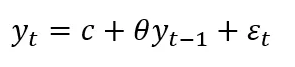
\includegraphics[width=0.5\linewidth]{a2.png}
    \caption{a2 Model autoregresji\cite{mod2023}}
\end{figure}
To znaczy, zgodnie z modelem AR (1), zmienna y w czasie t jest równa stałej (c), plus zmienna w (t-1) pomnożona przez współczynnik plus błąd. Należy zauważyć, że stała „c” może być liczbą dodatnią, ujemną lub zerową.Jeśli chodzi o wartość teta, czyli współczynnik pomnożony przez y (t-1), może przyjmować różne wartości.

MODEL ARIMA, czyli AutoRegressive Integrated Moving Average, to bardziej zaawansowany model szeregów czasowych, który łączy w sobie trzy główne składniki: model autoregresji (AR), model średniej ruchomej (MA) i różnicowanie (I, od ang. Integrated) . Jest modelem powstalym na bazie ARMA. W przypadku braku różnicowania model przeksztalca sie w ARMA.\cite{Musz2012}

Metoda Naiwna
 Metoda naiwna – metoda prognostyczna dotycząca analizy szeregów czasowych bez tendencji.Metoda ta stosowana jest przy stałym poziomie zjawiska i niewielkich wahaniach przypadkowych
Zalety: 

    • prosta i łatwa do zrozumienia 
    
    • szybka i tania

Wady:

    • niska jakość prognoz 
    
    Jest to prognoza typu: "jutro będzie tak jak dziś"
 \cite{naiw2023}\cite{Shekh2018} 

Mogą być stosowane w przypadku stwierdzenia niewielkich wahań w szeregu zmiennej prognozowanej i wykorzystane w prognozowaniu krótkookresowym, obejmującym jeden okres naprzód. 
Metody naiwne są szybkie i tanie w zastosowaniu, jednak jakość prognoz wyznaczonych z ich użyciem jest zwykle niska.
Przykłady:sprzedaż przedsiębiorstwa w następnym  kwartale będzie na dotychczasowym poziomie,
zysk wzrośnie w tym samym stopniu co ubiegłym miesiącu.\cite{szer2009}

\begin{figure}[h!]
    \label{fig:a3}
    \centering 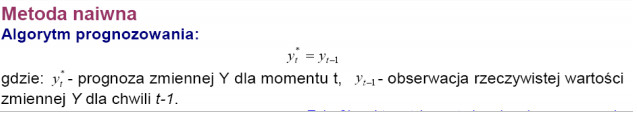
\includegraphics[width=0.8\linewidth]{a3.png}
    \caption{a3 Metoda naiwna\cite{szer2009}}
\end{figure}

Metoda sredniej ruchomej:  Polega na zastępowaniu danych empirycznych dla kolejnych okresów średnimi poziomami z okresu badanego i kilku okresów sąsiednich. Metoda średniej ruchomejmoże być 
stosowana zarówno do wygładzania szeregu czasowego, jak i do prognozowania.
\begin{figure}[h!]
    \label{fig:a4}
    \centering 
\includegraphics[width=0.8\linewidth]{a4.png}
    \caption{a4 srednia ruchoma algorytm\cite{szer2009}}
\end{figure}

Zalety: prosty algorytm, szybkie i tanie prognozowanie
Wady:koniecznosc doboru stalej K (min. ilosci błedów) dla duze K potrzeba trzymania duzej ilości danych
Dla usprawnienia dzialania mozna dodac czynnik wag do algorytmu to znaczy ze okres maja rozną wartośc (troche komplikuje algorytm).
Jest to prognoza krótkookresowa, typowa stacjonarna  gdzie zakladamy ze prognozowany okres bedzie podobny ostatnich k - okresów\cite{szer2009}
\begin{figure}[h!]
    \label{fig:a5}
    \centering 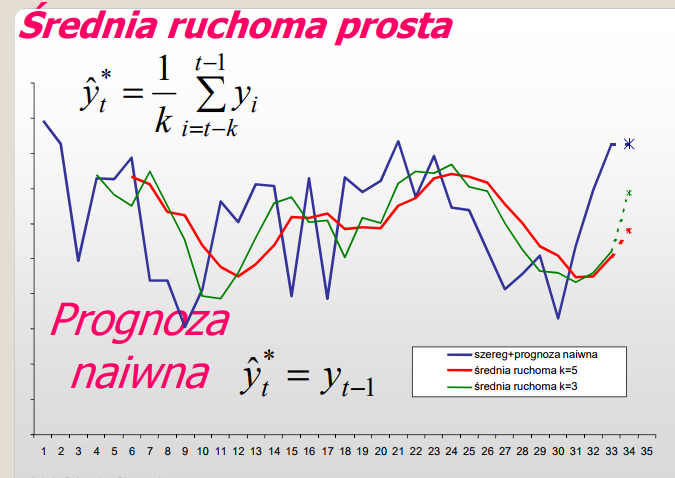
\includegraphics[width=0.8\linewidth]{a5.png}
    \caption{a5 srednia ruchoma wykres\cite{szer2009}}
\end{figure}



Model wykladzania wykładniczego.
Wygładzanie wykładnicze (ang. exponential smoothing) – metoda obróbki szeregu czasowego zmniejszająca jego wariancję za pomocą ważonej średniej ruchomej z przeszłych wartości, o wagach malejących wykładniczo wraz z odległością w czasie. Stosowana do prostego usuwania szumu(Stosunek sygnału do szumu (SNR, ang. signal-to-noise ratio) – miara porównująca poziom sygnału użytecznego (informacja) do poziomu szumu tła (niepożądany sygnał). Jest definiowana jako stosunek mocy sygnału użytecznego do mocy szumu tła i jest często wyrażona w decybelach (dB). ) . Jest przydatna w prognozowaniu szeregów czasowych o niewielkim stosunku sygnału do szumu, szczególnie niemających wyraźnego trendu i wahań sezonowych. \cite{wyg2023}

Jest rozszerzeniem idei średniej ruchomej i polega na:wygładzeniu oryginalnego szeregu tak, jak robi to średnia ruchoma ,użycia otrzymanego szeregu do uzyskania przyszłych wartości 
zmiennej, Istotne jest zwiększenie wpływu ostatnich wartości szeregu na 
prognozę, w stosunku do wpływu bardziej odległych obserwacji ,Największa waga jest nadana bieżącej obserwacji, mniejsza waga poprzedniej obserwacji i tak dalej. Wagi zmniejszają się 
geometrycznie w miarę cofania się w czasie. Jest to prosty i szybki algorytm typowy do danych stacjonarnych i nadaje sie na krotkookresowe prognozy\cite{szer2009}


\begin{figure}[h!]
    \label{fig:a6}
    \centering 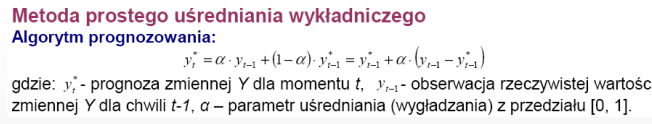
\includegraphics[width=0.8\linewidth]{a6.png}
    \caption{a6 Wygładzanie wykładnicze algorytm\cite{szer2009}}
\end{figure}


Kolejna grupa metod to wlączajace w prognoze trend naleza do nich:  metoda liniowa Holta, modele analityczne i adaptacyjne

Model Holta

Model Holta stosujemy wygładzając szereg czasowy, w którym wyróżnić można zarówno trend (tendencję rozwojową) jak i wahania przypadkowe.  występuja dwa parametry: alfa i beta.\cite{hol2023}

Model Holta pozwala na wygładzanie szeregu czasowego, w którym występuje tendencja rozwojowa oraz wahania przypadkowe. Wartości prognozowanego szeregu zostały oznaczone symbolami x0, x1, ..., xn-1. Model ten ma dwa parametry alfa oraz beta i następującą postać:
\begin{figure}[h!]
    \label{fig:a7}
    \centering 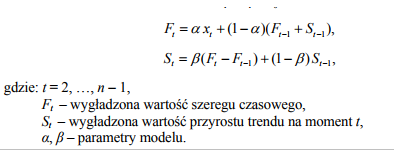
\includegraphics[width=0.8\linewidth]{a7.png}
    \caption{a7 Model Holta  obliczanie składnikow szeregu czasowego i trendu\cite{szos2012}}
\end{figure}

Parametry modelu Holta alfa oraz beta są dobierane tak, aby zminimalizować błędy prognoz\cite{szos2012}

Podwójne wygładzanie wykładnicze –Metoda HOLTA Przystosowane do szeregów czasowych ze składnikami 
sezonowymi i trendami.  Ogólna idea polega na tym, że prognozy są obliczane nie tylko 
na podstawie kolejnych poprzednich obserwacji (jak w prostym  wyrównywaniu wykładniczym), ale można także dodać niezależny trend i składnik sezonowy. 
 Wiele empirycznych szeregów czasowych zawiera wahania 
sezonowe. (np. roczna sprzedaż komputerów osiąga prawdopodobnie szczyt w listopadzie i grudniu i być może latem) Wzorzec ten będzie się prawdopodobnie powtarzał co roku, chociaż względna wielkość wzrostu sprzedaży w grudniu może się powoli zmieniać z roku na rok.Metoda nadaje sie do krotkookresowej prognozy. Zalety elastycznosc zas  wady trudnosc doboru parametrow\cite{szer2009}

\begin{figure}[h!]
    \label{fig:a8}
    \centering 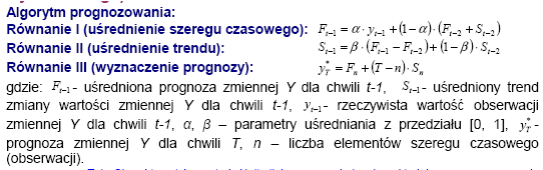
\includegraphics[width=0.8\linewidth]{a8.png}
    \caption{a8 Model Holta  cały algorytm\cite{szer2009}}
\end{figure}


Kolejny przyklad: Potrójne wygładzanie wykładnicze Metoda Wintersa
Model Holta-Wintersa działa na zasadzie „wygładzania” danych szeregów czasowych za pomocą trzech równań wygładzania: dla poziomu, trendu i sezonowości. W efekcie model jest w stanie uwzględnić zmiany zarówno w trendzie, jak i w sezonowości, dostarczając dokładniejsze prognozy.\cite{exc2018}
Model Wintersa może być stosowany w przypadku szeregów czasowych zawierających tendencję rozwojową, wahania sezonowe oraz wahania przypadkowe. \cite{win2023}

\begin{figure}[h!]
    \label{fig:a9}
    \centering 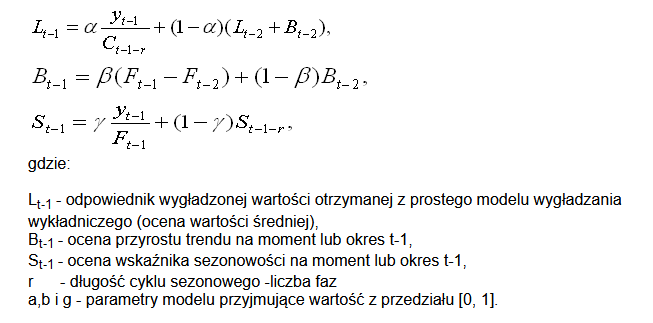
\includegraphics[width=0.8\linewidth]{a9.png}
    \caption{a9 Model Wintersa  obliczane składniki \cite{win2023}}
\end{figure}

pelny algorytm:

\begin{figure}[h!]
    \label{fig:a10}
    \centering 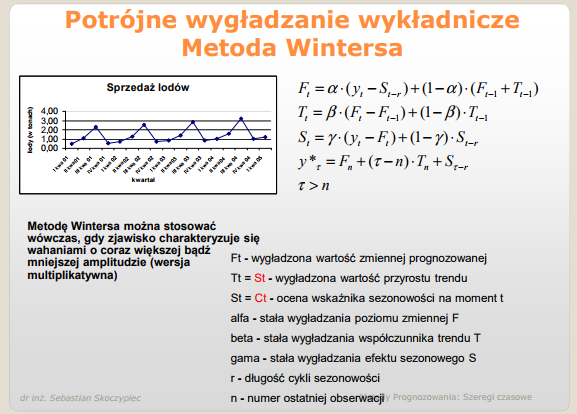
\includegraphics[width=0.8\linewidth]{a10.png}
    \caption{a10 Model Wintersa  pelny algorytm \cite{szer2009}}
\end{figure}

\newpage

\paragraph{Algorytmy uczenia maszynowego}


w skróce w maszynowym uczeniu mozna wyodrebnic
Uczenie nadzorowane (ang. supervised learning) – sposób uczenia, w którym zbiór danych treningowych, na których uczy się algorytm, zawiera dołączone rozwiązanie problemu, tzw. etykiety albo klasy. 

Uczenie nienadzorowane(ang. unsupervised learning) – sposób uczenia modelu, w którym dane uczące są nieoznakowane tzn. nie posiadają etykiet. Mówiąc potocznie, posiadamy surowe dane które wrzucamy do modelu i zostawiamy algorytmowi całą pracę wiązaną ze znalezieniem powiązań między danymi (tzw. uczenie bez nauczyciela).

Uczenie przez wzmacnianie(ang. RL - reinforcement learning) – jeden z trzech głównych nurtów uczenia maszynowego, którego zadaniem jest interakcja ze środowiskiem na podstawie zebranych informacji. W przeciwieństwie do wymienionych wcześniej rodzajów, w uczeniu przez wzmacnianie nie przygotowuje się zestawu danych uczących, tylko środowisko, z którego model będzie zbierał dane automatycznie. 

  Uczenie półnadzorowane(ang. semisupervised learning) – algorytmy działające na częściowo oznakowanych danych\cite{gove2023}

 Algorytmy prognozowania ML często wykorzystują techniki obejmujące bardziej złożone cechy i metody predykcyjne, ale cel metod prognozowania ML jest taki sam, jak w przypadku metod tradycyjnych – poprawa dokładności prognoz przy jednoczesnej minimalizacji funkcji straty. Funkcję straty przyjmuje się zwykle jako sumę kwadratów spowodowaną błędami w przewidywaniu/prognozowaniu. Najważniejsza różnica pomiędzy obiema metodami polega na sposobie minimalizacji. Chociaż większość tradycyjnych metod wykorzystuje wyjaśnialne procesy liniowe, większość metod ML wykorzystuje techniki nieliniowe w celu minimalizacji funkcji strat. 



Oto kilka przykładów modeli prognozowania uczenia maszynowego stosowanych w aplikacjach biznesowych:
    • Artificial neural network
    • Long short-term-memory-based neural network
    • Random forest
    • Generalized regression neural networks
    • K-nearest neighbors regression
    • Classification and regression trees (CART)
    • Support vector regression
    • Gaussian processes 
\cite{gen2023}


w literaturze poswieconej stosowaniu maszynowego uczenia w prognozowaniu popytu spotkalem sie ze najczesciej stosowane modele do prognozowania popytu to:

Neural Networks (NN), zwane również sztucznymi sieciami neuronowymi, są inspiracją biologicznych neuronów. Składają się z warstw neuronów (lub węzłów), które przetwarzają dane i przekazują informacje między sobą za pomocą wag.

Recurrent Neural Networks (RNN) to rodzaj sieci neuronowych, które posiadają pętle rekurencyjne, które pozwalają im na uwzględnianie informacji z poprzednich kroków czasowych w analizie sekwencji danych..

Support Vector Machines (SVM) to technika uczenia maszynowego stosowana zarówno do zadań klasyfikacji, jak i regresji.Tutaj jest wybieranna hiperpłaszczyzne decyzyjna które najlepiej oddziela klasy i pozwala prognozowac (na podstawie danych treningowych i cech), optymalizy=uje margines (miedzy najblizszymi punktami danych a hiperplaszczyzna- wektory nosne), uzywa funkcje jadrowe ktore umowzliwaja przeksztalcanie danych do wyzszych wymiarow/przestszeni gdzie zostaja liniowo odseparowane (mimo ze zaleznosci nie sa liniowe). Najbardziej popularne to :  RBF (Radial Basis Function) i funkcja wielomianowa. Dobierane sa parametry np bledu ktore powoduja zwiekszenia lub zmniejszenie czulosci na dokladnosc( czasami warto dopuscic pewna ilosc bledow niektore dane sa 'wyjatkami')

dodatkowo z KNN (K najbliższych sąsiadów)  jeden z algorytmów regresji nieparametrycznej używanych w statystyce do prognozowania wartości pewnej zmiennej losowej. Może również być używany do klasyfikacji. k-NN może być używane do prognozowania popytu poprzez identyfikowanie podobnych wzorców historycznego popytu do obecnej sytuacji.używamy dane historyczne dotyczących popytu jako zestawu treningowego. Każdy punkt danych reprezentuje przeszły wzorzec popytu i zawiera cechy takie jak pora roku, promocje,  itp. Gdy chcesz prognozować przyszły popyt, obliczasz podobieństwo (odległość) między obecną sytuacją a k-najbliższymi historycznymi wzorcami popytu.

Drzewo decyzyjne,jest intuicyjnym narzędziem do prognozowania, które pozwala na interpretację wyników i jest często używane w analizie danych i uczeniu maszynowym. są często stosowane w prognozowaniu popytu, aby uwzględnić hierarchiczną strukturę czynników wpływających na popyt.
Jak to działa: Buduje drzewo decyzyjne na podstawie danych historycznych, gdzie popyt jest zmienną docelową, a różne czynniki (np. cena, wydatki , sezonowość) są cechami wejściowymi. Drzewo jest budowane poprzez rekurencyjne dzielenie danych na podzbiory na podstawie najważniejszej cechy, aż zostaną spełnione kryteria zatrzymania.

wszystkie one dziela dane na zbiur uczacy i testowy, dla kazdego z nich bardzo waza jest jakosc danych ktore sie wprowadza, odpowiednie oznaczanie cech, żaden z nich nie bedzie dobrze dzialal jest zostana wrpowadzone do uczenia dane złej jakości.Dobór danych do uczenia ma bezposredni wpływ na dzialanie kazdego agorytmu ML.

Np. SVM bardzo dobrze radzi z wieloma czynnikami.Zdolność do radzenia sobie z danymi o wielu wymiarach: SVM są skuteczne w przekształcaniu danych do przestrzeni o wysokiej liczbie wymiarów.Efektywnoe radzi sobie z danymi nieliniowymi: SVM mają wbudowaną zdolność do radzenia sobie z danymi nieliniowymi, dzięki zastosowaniu funkcji jądrowych, które pozwalają na transformację danych do przestrzeni o wyższej wymiarowości, gdzie mogą być liniowo separowalne.
RNN i NN jak i SVM dobrze radza sobie ze skomplikowanymi danymi, nieliniowymi zaleznosciami,dla RNN. Nieliniowość jest jednym z kluczowych atutów modeli maszynowego uczenia nad tradycyjnymi modelami opartymi o szeregi czasowe.Oto dlaczego nieliniowość jest główną zaletą tych modeli:Zdolność do modelowania skomplikowanych zależności: W rzeczywistych problemach, zależności między danymi często są skomplikowane i nieliniowe.Zdolność do rozwiązywania problemów klasyfikacji nieliniowej: W zadaniach klasyfikacji, gdzie celem jest podział danych na różne klasy, istnieją sytuacje, w których granica decyzyjna między klasami nie jest liniowa.Zdolność do wydobywania nieliniowych wzorców w danych: W przypadku analizy danych, często istnieją nieliniowe wzorce lub zależności, które mogą być trudne do wykrycia za pomocą tradycyjnych modeli liniowych. Elastyczność w dostosowywaniu się do danych: Modele nieliniowe pozwalają na bardziej elastyczne dopasowanie do różnych rodzajów danych

Wsteczna propagacja błędu w czasie, pozwala na uczenie się wzorców na dowolnej głębokości
w szeregu czasowym. Sama wstepna propagacja pomaga na biezaco dopasowywac model: Wsteczna propagacja błędu w czasie (ang. Backpropagation Through Time, BPTT) to technika uczenia sieci RNN poprzez dostosowywanie wag na podstawie błędów prognoz w kolejnych krokach czasowych. Pozwala to na aktualizację wag w sieci, aby minimalizować błąd prognozowany przez model.


Dla oceny jakosc  czesto stosuje sie MAPE.
MAPE (Mean Absolute Percentage Error) to popularna metryka używana do oceny jakości prognoz w problemach prognozowania popytu lub innych zadań regresji. MAPE pozwala na ocenę dokładności prognoz w sposób procentowy, co jest szczególnie przydatne do porównywania prognoz między różnymi zestawami danych lub modelami.

\begin{figure}[h!]
    \label{fig:a11}
    \centering 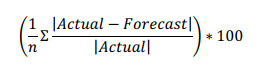
\includegraphics[width=0.8\linewidth]{a11.png}
    \caption{a11 MAPE \cite{Shekh2018}}
\end{figure}

\cite{carb2006}\cite{Mary2022}\cite{wikknn2023}\cite{Shekh2018}\cite{Xiao2021}\cite{Resul2017}


\newpage
\subsubsection{Optymalizacja zapasów}

\paragraph{Wprowadzenie}

Optymalizacja zapasów (zarządzanie zapasami) polega na skutecznym zarządzaniu ilościami produktów przechowywanych w magazynach. Głównym celem jest zminimalizowanie kosztów magazynowania, jednocześnie zapewniając wystarczający poziom dostępności produktów, aby zaspokoić popyt klientów. Tradycyjne metody zarządzania zapasami, takie jak metoda ABC czy metoda EOQ (Economic Order Quantity), są stosunkowo statyczne i nie uwzględniają zmienności popytu i innych czynników.
Samo zarządzanie zapasami spupia sie na 4 kwestiach:
Koncentruje się na czterech zasadniczych kwestiach:

   - ile jednostek należy zamówić (lub wyprodukować) w danym czasie,
   
   - kiedy należy złożyć zamówienie,
   
  -  które składniki zapasów wymagają szczególnej uwagi,
  
 -   czy można zabezpieczyć się przed wzrostem kosztów zapasów.

  Głowne metody stosowane to
  
 - Reguła 80/20 - na jej bazie została stworzona metodyka ABC, dzieli zapasy pod kątem wartości. Skoro 20 procent pozycji stanowi 80procent całkowitej wartości zapasu, to sugeruje odmienne podejście do sterowania zapasem tych 20procent pozycji, do procesu wyboru dostawców oraz do obsługi dostaw.

 - Metoda ABC polegająca na podziale zapasów na trzy grupy. Podział ten oparty jest na założeniu, że zapasy, które ilościowo stanowią duży udział w zapasach ogółem, lecz mały pod względem wartościowym. I odwrotnie: są też takie zapasy, których udział wartościowy jest duży, a mały ilościowo. Dzieli materiały (lub wytwarzane produkty) na ważne, mniej ważne i nieważne. 
 
-Metoda XYZ(metoda ilościowa) jest uzupełnieniem metody ABC, w której zapasy rozpatruje się z punktu widzenia regularności zapotrzebowania i dokładności prognozowania. Klasa X zawiera asortymenty, na które występuje regularne zapotrzebowanie (popyt). Klasa Y stanowi asortyment, na który występują sezonowe wahania w zapotrzebowaniu. Klasa Z składa się z asortymentu, na który występuje sporadyczne (okazjonalne) zapotrzebowanie. 

-Model ekonomicznej (optymalnej) wielkości zamówienia - EOQ (Economic Order Quantity) jest najbardziej rozpowszechnioną koncepcją wykorzystywaną w zarządzaniu zapasami materiałów i towarów. Wraz ze wzrostem wielkości zamówienia wzrasta poziom przeciętnych zapasów, a to z kolei powoduje spadek kosztów tworzenia i wzrost kosztów utrzymania zapasów. Jeżeli natomiast częstotliwość zamówień się zwiększy, to wielkość przeciętnych zapasów spadnie, zmniejszą się także koszty utrzymania, a wzrosną koszty tworzenia zapasów. 

-Metoda "dokładnie na czas" (just- in- time JIT) polega na tym że, system gospodarki zapasami, w którym niezbędne materiały wpływają dokładnie wtedy, kiedy są potrzebne, bez zakłóceń procesu produkcji, co pomaga organizacji kontrolować zapasy surowców, ograniczając zapotrzebowanie na powierzchnię magazynową. System ten zmniejsza zakres niezbędnych nakładów organizacji na przestrzeń magazynową potrzebna do przechowywania materiałów i na same materiały. Polega ona na również na zamawianiu materiałów i części, w mniejszych partiach, zmniejszając tym samym nakłady na przestrzeń magazynową oraz nakłady zamrożone w samych zapasach. 


Koszty zapasow mozemy podzielic na 3 czesci:


   - koszty tworzenia zapasów,
   
   - koszty utrzymania zapasów,
    
  -koszty niedoboru zapasów.
 
\cite{enc2023}\cite{Prav2020}


\paragraph{Wykorzystanie uczenia maszynowego w optymalizacji zapasów}
'stare' metody sa statyczne nie uwzgledniaja zmian, opieraja sie kilku max kilku cechach (zazwyczaj 2 cechy: cena, zapotzebowanie) jakiekolwiek zmiany wymagaja duzej pracy ludzkiej, nie dostosowuja sie do zmian, nie sa elastyczne, nie radza sobie z duza iloscia danych, . ML ten sam akgorytm moze pracowac zarowno dla malej jak i duzej firmy dla kazdego produktu, pod produktu, polproduktu jak i rodzin produktowych (tam gdzie armia ludzi w biurze i magazynie jest potrzebna do obslugi uzywajac tradycyjnych metod). Były wykorzystywane przez kilkadziesiat lat ale mozliwosci jakie daje maszynowe uczenie pozwala na usprawnienie pracy

Maszynowe Uczenie oferuje:

Dopasowanie do zmiennego popytu: W przeciwieństwie do tradycyjnych metod, które zakładają stałe lub statystyczne wartości (np. stałą wielkość zamówienia w EOQ), algorytmy uczenia maszynowego są w stanie dostosowywać się do zmiennej natury popytu. Mogą analizować historyczne dane sprzedaży i innych czynników wpływających na popyt, co pozwala na generowanie dokładniejszych prognoz

Real-time reakcje: Uczenie maszynowe pozwala na monitorowanie i dostosowywanie poziomów zapasów w czasie rzeczywistym. Gdy zmieniają się warunki rynkowe, takie jak sezonowość, trendy konsumenckie lub zmiany w dostawach, algorytmy ML mogą reagować szybciej niż statyczne metody.

Automatyzacja zamawiania ,Sztuczna inteligencja zapewnia przewagę w postaci automatycznego ponownego zamawiania, czyli funkcji, która może znacznie poprawić efektywność zapasów. Na podstawie przewidywania trendów sprzedaży i aktualnych poziomów zapasów sztuczna inteligencja może we właściwym czasie uruchamiać automatyczne zamówienia uzupełniające, zapewniając w ten sposób optymalny poziom zapasów.

Analiza wielu czynników: ML może uwzględniać wiele czynników jednocześnie. Oprócz historii sprzedaży może analizować dane meteorologiczne, trendy konsumenckie, promocje , zmiany cen i wiele innych. Dzięki temu może lepiej zrozumieć, co wpływa na popyt i dostosować się do tych zmian.

Zwiększona precyzja: ML może dostarczyć bardziej precyzyjne prognozy popytu, co pomaga w uniknięciu nadmiarowych zapasów (które generują koszty magazynowania) lub braków w dostawach (co wpływa na obsługę klienta i straty finansowe).

Wykrywanie anomalii: Algorytmy uczenia maszynowego są również zdolne do wykrywania anomalii w danych magazynowych, co pozwala na szybkie reagowanie na nieprawidłowości w poziomach zapasów.

Personalizacja: ML może dostosowywać strategie zarządzania zapasami do konkretnych rodzajów produktów, co pozwala na bardziej efektywne podejście w zależności od charakterystyki produktów.
\cite{linn2023}\cite{cdp2023}\cite{Matti2023}\cite{Had2023}

W literaturze spotykam ponizsze algorytmy maszynowego uczenia stosowane do optymalizacji zapasów:
SVM, SVR, RNN, ANN, drzewa decyzyjne, Q-Learning. wiekszosc z nich została juz skrótowo opisana w poprzednim podrozdziale. Tutaj na uwahe zasługuje jeszce nie opisywany SVR i Q-Learning

SVR (Support Vector Regression) to algorytm uczenia maszynowego wykorzystywany do rozwiązywania problemów regresji, czyli przewidywania wartości numerycznych na podstawie danych treningowych. Działa on na podobnej zasadzie co SVM (Support Vector Machine) w przypadku klasyfikacji, ale jest dostosowany do problemów regresji zas SWM klasyfikuje dane i je dzieli.Regresja to pojęcie w statystyce i analizie danych, które odnosi się do procesu modelowania zależności między jedną lub wieloma zmiennymi niezależnymi (czynnikami) a zmienną zależną (wartością, którą chcemy przewidzieć). Głównym celem regresji jest znalezienie matematycznego modelu lub funkcji, która opisuje, jak zmienne niezależne wpływają na zmienną zależną.

Q-Learning to algorytm uczenia maszynowego, który jest często wykorzystywany do uczenia się optymalnych strategii w problemach decyzyjnych z uczeniem ze wzmocnieniem.Ogólna idea Q-Learning polega na uczeniu agenta, jakie akcje podejmować w danej sytuacji, aby maksymalizować sumę nagród na przestrzeni wielu kroków czasowych. Algorytm ten jest często używany w kontekście gier i problemów, w których agent interaktywnie działa w pewnym środowisku.Oto główne kroki algorytmu Q-Learning: 

-Inicjalizacja tabeli Q: Tworzona jest tabela (lub macierz) Q, która przechowuje wartości Q dla wszystkich dostępnych stanów i akcji.

- Wybór akcji: Agent rozpoczyna w pewnym stanie środowiska. Na podstawie wartości Q wybierana jest akcja, którą agent chce podjąć. Może to być akcja wybrana w sposób zachłanny (na podstawie maksymalnej wartości Q) 

- Wykonanie akcji: Agent wykonuje wybraną akcję i przechodzi do nowego stanu środowiska.

-Obserwacja nagrody i nowego stanu: Agent obserwuje, ile nagrody otrzymuje za podjętą akcję oraz jaki jest nowy stan środowiska, do którego przeszedł.

-Aktualizacja wartości Q: Wartość Q dla danej pary stanu i akcji jest aktualizowana na podstawie otrzymanej nagrody i przewidywanej przyszłej wartości Q. Istnieje wiele czynników, które sprawiają, że Q-learning ma kluczowe znaczenie:

Dlaczego używamy q-learning? Po pierwsze, bez wyraźnego programowania komputery mogą uczyć się na nowych ustawieniach i dostosowywać się do nich. Nazywa się to Q-learningiem. Należałoby napisać wyraźne instrukcje dla każdej istotnej okoliczności, z jaką może spotkać się komputer w tradycyjnym programowaniu. Komputer jest bardziej wszechstronny i dostosowuje się do nowych scenariuszy dzięki Q-learningowi, który pozwala mu na samodzielną naukę metodą prób i błędów.
Po drugie, różnorodne procesy decyzyjne, w tym te w robotyce, teorii gier i finansach, można zoptymalizować za pomocą Q-learningu. Q-learning może pomóc komputerom w dokonywaniu bardziej przydatnych ocen w skomplikowanych kontekstach poprzez identyfikację najlepszego sposobu działania lub zbioru działań, które maksymalizują długoterminową nagrodę.

Odnosnie zarzadzania zapasami, q-learning jest wstanie podejmowac decyzje co zamowic kiedy ile, po jakiej cenie jest wstanie podejmowac optymalne decyzje w srodowisku ktore jest dynamiczne, ma bardzo duzo danych , dzieki permanentnej eksploracji ten model jest wstanie osiagnac znacznie wiecej niz czlowiek z tradycyjnymi modelami. Monza bez problemu wprowadzic toczenie dla agenta gdzie beda koszt zamawiania, koszt zakupu, koszt trzymania materialu, przychod ze sprzedazy, koszt braku materiału na stanie itp...

\cite{Had2023}\cite{wiksvr2023}\cite{alakh2023}\cite{intell2023}



\paragraph{Kolejny poziom podsekcji}

\newpage
\subsubsection{Planowanie produkcji}

\newpage
\par
\subsection{Kluczowe algorytmy uczenia maszynowego dla łańcucha dostaw}
    W ostatnim rozdziale z tej sekcji prezentujemy kluczowe algorytmy uczenia maszynowego, które są szczególnie istotne dla zarządzania łańcuchem dostaw. Opisujemy, jak działają te algorytmy i w jakich przypadkach mogą być używane. Wśród omawianych algorytmów znajdują się między innymi regresja liniowa, drzewa decyzyjne, sieci neuronowe, maszyny wektorów nośnych oraz algorytmy klastrowania. Dla każdego algorytmu przedstawiamy także przykłady jego potencjalnych zastosowań w SCM.
Celem tych rozdziałów jest zaprezentowanie czytelnikowi podstawowych informacji na temat maszynowego uczenia i jego roli w zarządzaniu łańcuchem dostaw oraz dostarczenie wglądu w kluczowe algorytmy, które mogą być używane do rozwiązywania problemów związanych z SCM.




\subsubsection{Klastrowanie}

 Np. grupowanie/klastrowanie (clustering) jest jednym z metod sztucznej inteligencji.Grupowanie, znane również jako klasyfikacja lub analiza skupień, to technika przetwarzania danych wykorzystywana w dziedzinie uczenia maszynowego i sztucznej inteligencji. Polega na dzieleniu zbioru danych na grupy (skupienia) na podstawie podobieństwa między jego elementami. W analizie danych i uczeniu maszynowym termin "clustering" jest szeroko używany i odnosi się do procesu tworzenia grup (klas) obiektów na podstawie pewnych kryteriów, takich jak odległość między obiektami. Celem jest stworzenie skupisk obiektów, które są podobne do siebie wewnątrz klastra, ale różnią się od obiektów w innych klastrach.Istnieje cały szereg algorytmow zastosowan klastrowania w sztucznej inteligencji.

  Klastrowanie to dla uczenia maszynowego nienadzorowanego. Możesz również usłyszeć, że nazywa się to analizą skupień ze względu na sposób działania tej metody.Użycie algorytmu grupowania oznacza, że dasz algorytmowi dużo danych wejściowych bez etykiet i pozwolisz mu znaleźć dowolne grupy w danych, jakie tylko może.Grupy te nazywane są klastrami. Klaster to grupa punktów danych, które są do siebie podobne na podstawie ich relacji do otaczających punktów danych.Kiedy zaczynasz od danych, o których nic nie wiesz, klastrowanie może być dobrym miejscem na uzyskanie wglądu.Istnieją różne typy algorytmów grupowania:
  
 •  Oparte na gęstości.W klastrowaniu opartym na gęstości dane są grupowane według obszarów o dużej koncentracji punktów danych otoczonych obszarami o niskiej koncentracji punktów danych. Zasadniczo algorytm znajduje miejsca gęste z punktami danych i wywołuje te klastry.

 •  Oparta na dystrybucji.W przypadku podejścia klastrowego opartego na dystrybucji wszystkie punkty danych są uważane za części klastra na podstawie prawdopodobieństwa, że należą do danego klastra.Działa to w ten sposób: istnieje punkt środkowy i wraz ze wzrostem odległości punktu danych od środka maleje prawdopodobieństwo, że będzie on częścią tego klastra.

  •  Oparty na centroidach.Jest trochę wrażliwy na parametry początkowe jakie mu podajesz, ale jest szybki i wydajny.Algorytmy tego typu oddzielają punkty danych na podstawie wielu centroidów w danych. Każdy punkt danych jest przypisany do klastra na podstawie kwadratu odległości od środka ciężkości. Jest to najczęściej stosowany rodzaj grupowania.
  
  •  Oparte na hierarchii.Klastrowanie oparte na hierarchii jest zwykle używane w przypadku danych hierarchicznych, takich jakie można uzyskać z firmowej bazy danych lub taksonomii. Buduje drzewo klastrów, dzięki czemu wszystko jest zorganizowane od góry do dołu.\cite{clust2020}

Najbardziej znane algorytmy sztucznej inteligencji bazujaca na klastrowaniu to:
  • Algorytm grupowania K-średnich(K-means).Grupowanie K-średnich jest najczęściej używanym algorytmem grupowania. Jest to algorytm oparty na centroidach i najprostszy algorytm uczenia się bez nadzoru.Algorytm ten próbuje zminimalizować wariancję punktów danych w klastrze. Średnie K najlepiej stosować w przypadku mniejszych zestawów danych, ponieważ iterują po wszystkich punktach danych. Oznacza to, że klasyfikacja punktów danych zajmie więcej czasu, jeśli w zbiorze danych znajduje się ich duża liczba.\cite{clust2020}

Jest to iteracyjny proces przypisywania każdego punktu danych do grup, w wyniku którego punkty danych są powoli grupowane w oparciu o podobne cechy. Celem jest zminimalizowanie sumy odległości między punktami danych a środkiem ciężkości klastra, aby zidentyfikować właściwą grupę, do której powinien należeć każdy punkt danych.Tutaj dzielimy przestrzeń danych na K klastrów i przypisujemy każdemu z nich średnią wartość. Punkty danych są umieszczane w skupieniach najbliższych średniej wartości tego skupienia. Dostępnych jest kilka wskaźników odległości, które można wykorzystać do obliczenia odległośc.
Jak działają K-średnie?
Weźmy przykład, aby zrozumieć, jak krok po kroku działają K-średnie. Algorytm można podzielić na 4-5 kroków.


    A. Wybór liczby klastrów
Pierwszym krokiem jest zdefiniowanie liczby K skupień, w których będziemy grupować dane. Wybierzmy K=3.

    B. Inicjowanie centroidów
Centroid jest środkiem klastra, ale początkowo dokładny środek punktów danych będzie nieznany, dlatego wybieramy losowe punkty danych i definiujemy je jako centroidy dla każdego klastra. Zainicjujemy 3 centroidy w zbiorze danych.

\begin{figure}[h!]
    \label{fig:k1}
    \centering 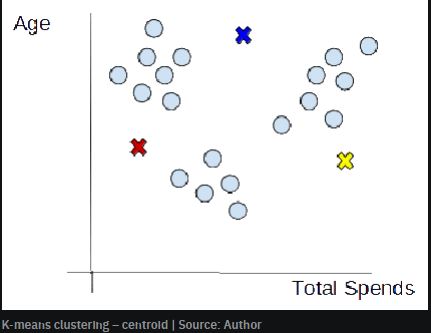
\includegraphics[width=0.8\linewidth]{K1.png}
    \caption{k1 Grupowanie K-średnich\cite{clust2020}}
\end{figure}
 \newpage
 C.Przypisz punkty danych do najbliższego klastra
Teraz, gdy centroidy zostały zainicjowane, następnym krokiem jest przypisanie punktów danych Xn do ich najbliższego środka ciężkości klastra Ck
\begin{figure}[!h]
    \label{fig:k2}
    \centering 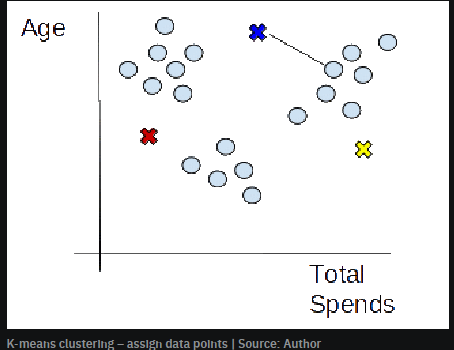
\includegraphics[width=0.8\linewidth]{K2.png}
    \caption{k2 Grupowanie K-średnich przypisanie danych\cite{clust2020}}
\end{figure}

W tym kroku najpierw obliczymy odległość między punktem danych X a środkiem ciężkości C, korzystając z metryki odległości euklidesowej.
Metryka odległości euklidesowej:
\begin{figure}[h!]
    \label{fig:k3}
    \centering 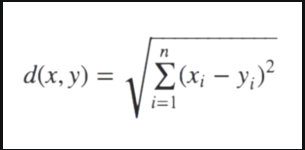
\includegraphics[width=0.5\linewidth]{K3.png}
    \caption{k3 Metryka odległości euklidesowej.Wzór\cite{clust2020}}
\end{figure}
\\
\\

Następnie wybierz klaster dla punktów danych, w których odległość między punktem danych a środkiem ciężkości jest minimalna.
\begin{figure}[h!]
    \label{fig:k4}
    \centering 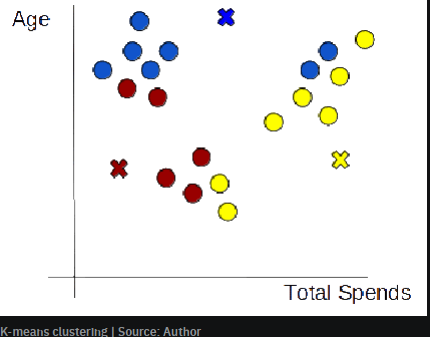
\includegraphics[width=0.5\linewidth]{K4.png}
    \caption{k4 Grupowanie K-średnich,dane przypisane do klastrów\cite{clust2020}}
\end{figure}
  
    D.  Zainicjuj ponownie centroidy
Następnie ponownie zainicjujemy centroidy, obliczając średnią wszystkich punktów danych tego klastra.
\begin{figure}[!h]
    \label{fig:k5}
    \centering 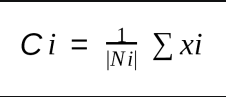
\includegraphics[width=0.4\linewidth,height=2cm]{K5.png}
    \caption{k5 Obliczamy centroide.Wzór\cite{clust2020}}
\end{figure}

\begin{figure}[!h]
    \label{fig:k6}
    \centering 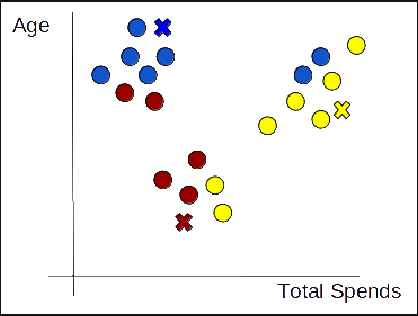
\includegraphics[width=0.6\linewidth,height=4cm]{K6.png}
    \caption{k6 Grupowanie K-średnich,dane przypisane do klastrów\cite{clust2020}}
\end{figure}
\newpage
     E.Powtórz kroki 3 i 4

Będziemy powtarzać kroki 3 i 4, aż uzyskamy optymalne centroidy, a przypisanie punktów danych do odpowiednich klastrów nie będzie się już zmieniać.
\begin{figure}[!h]
    \label{fig:k7}
    \centering 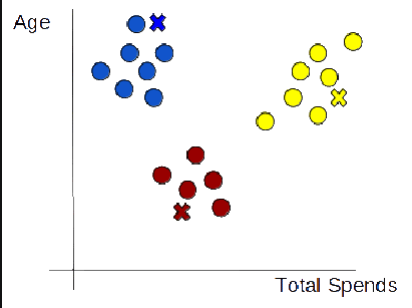
\includegraphics[width=0.5\linewidth, height=5cm]{K7.png}
    \caption{k7 Grupowanie K-średnich,dane przypisane do klastrów\cite{clust2020}}
\end{figure}

Does this iterative process sound familiar? Well, K-means follows the same approach as Expectation-Maximization(EM). \cite{clust2020}

\newpage


